\chapter{Résultats}

\section{Tests d'indépendance statistique}

Je présente ici les résultats obtenus en utilisant la méthode de représentation symbolique par canaux, pour deux sujets, un de la tâche visuelle et un de la tâche auditive, selectionnés de manière aléatoire. Pour chaque ensemble d'époques relatives à une condition expérimentale, on extrait des représentations symboliques dont on estime le taux d'entropie grâce à l'estimateur de Lempel-Ziv. On obtient alors une matrice contenant le taux d'entropie les séquences symboliques extraites à partir de segments temporels d'intérêt des canaux du signal MEG (ce sont les lignes de la matrice) et ce pour chaque époque (colonnes). Pour chaque canal, on calcule la médiane sur les époques que l'on garde. On a alors un vecteur contenant les taux d'entropie relatifs à chaque canal.

\vspace{2ex}
On décide d'effectuer des tests-t statistiques \cite{22} entre les vecteurs d'entropie associés à des conditions expérimentales différentes. Par exemple, on va comparer la mesure obtenue sur les target words au sein des phrases avec celle obtenue sur les target words au sein des listes aléatoires de mots.
Le test-t nous donne un résultat important, il nous informe si la différence observée entre les deux mesures est statistiquement significative.

\vspace{2ex}
Etant donné que nos mesures proviennent du même sujet, même s'il a été soumis à des stimuli différents, on peut donc considéré nos vecteurs d'entropie comme appariés. En effet, le test-t pour échantillons appariés peut être utilisé pour des sujets qui ont été exposés à deux conditions expérimentales. Les quantités que l'on compare sont des taux d'entropie qui constituent bien une mesure au sens mathématique du terme et l'on a utilisé la même métrique pour chaque condition expérimentale. 

\section{Interprétation des résultats}

On s'intéresse à la valeur p ou "p-value" comme résultat du test-t. Celle-ci nous donne la probabilité de l'hypothèse nulle, i.e., que les deux populations sont statistiquement identiques. Lorsque l'on obtient une valeur p inférieure à $5\%$, $p\geq 0.05$, on peut considérer que la probabilité de l'hypothèse nulle correspond au hasard et donc que les deux échantillons sont statistiquement différents.

On présente ici les résultats que nous avons obtenus en comparant les échantillons de taux d'entropie relatifs à différentes conditions expérimentales.

\subsection{Target word vs individual word}

\begin{figure}[!ht]
    \centering
    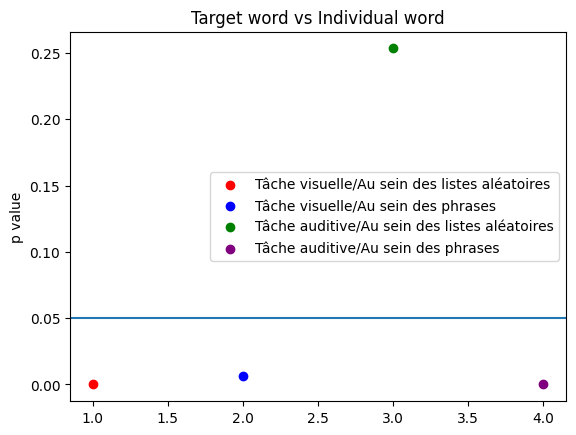
\includegraphics[width=10cm]{Targetword_vs_Individualword.png}
    \caption{Tests t apparayés entre les vecteurs d'entropie relatifs aux target words par rapport aux individual words}
    \label{fig6.1}
\end{figure}

On observe que pour la tâche visuelle, les dynamiques cérébrales associées aux target words et aux individual words sont statistiquement différentes, que ce soit au sein des phrases ou des listes aléatoires de mots. Pour la tâche auditive, les dynamiques cérébrales associées aux targets words et aux individual words sont statistiquement différentes au sein des phrases tandis qu'elles sont statistiquement différentes au sein des listes aléatoires de mots. On peut donc confirmer que pour la tâhce auditive, la dynamique cérébrale permet effectivement de distinguer des degrés de complexité linguistiques en lien avec des conditions expérimentales différentes.

\subsection{Phrases simples vs listes aléatoires de mots issues de phrases simples}

\begin{figure}[!ht]
    \centering
    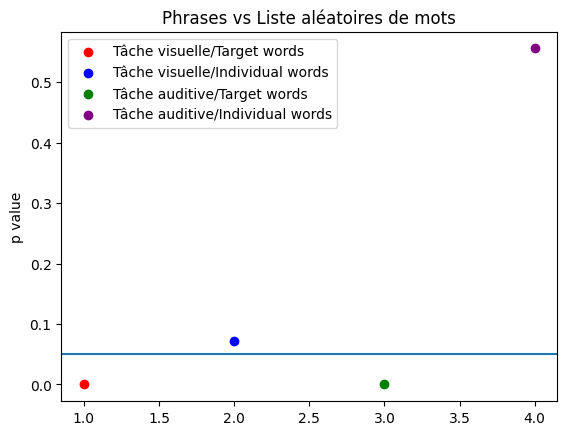
\includegraphics[width=10cm]{Phrases_vs_Listes_aleatoires.png}
    \caption{Tests t apparayés entre les vecteurs d'entropie relatifs aux phrases par rapport aux listes aléatoires de mots}
    \label{fig6.2}
\end{figure}

On retrouve ici ce que l'on a pu observer sur le graphique de résultats précédent. En effet, les target words semblent être les piliers de compréhension des phrases, ce qui permet d'indexer la complexité linguistique avec la dynamique cérébrale. En effet, les mesures de la dynamique cérébrale sont statistiquement différentes entre les phrases simples et les listes aléatoires de mots lorsque l'on s'intéresse aux targets words. Ce n'est pas le cas lorsque l'on se base sur les individual words, où les dynamiques cérébrales associées sont statistiquement semblables.

\subsection{Tâche visuelle vs tâche auditive}

\begin{figure}[!ht]
    \centering
    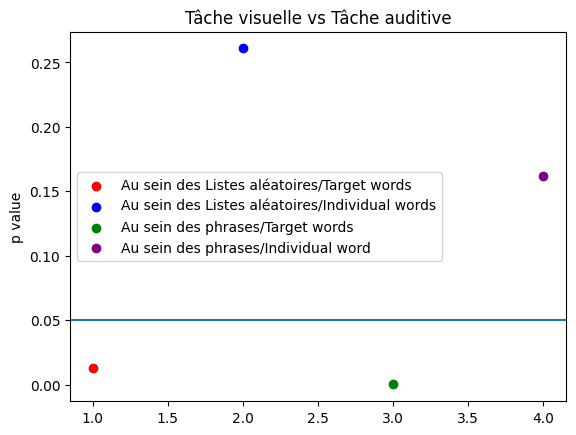
\includegraphics[width=10cm]{visuelle_vs_auditive.png}
    \caption{Tests t apparayés entre les vecteurs d'entropie relatifs à la tâche visuelle par rapport par rapport à la tâche auditive}
    \label{fig6.3}
\end{figure}

On observe que les dynamiques cérébrales associées à la tâche visuelle et auditive sont statistiquement différentes lorsque l'on se base sur les target words, que ce soit au sein des phrases ou bien des listes aléatoires de mots. Encore une fois, la compréhension linguistique auditive et visuelle ne s'opérant pas de la même manière, on peut les discriminer grâce à la dynamique cérébrale en se basant sur les target words, que ce soit au sein des phrases ou des listes aléatoires de mots. Comme on pouvoit s'y attendre, cette conclusion n'est pas possible lorsque l'on s'intéresse aux individual word. En effet, les dynamiques associées sont statistiquement semblables dans la tâche auditive comme dans la tâche visuelle.

\subsection{Récapitulatif des résultats des tests statistiques}

\begin{figure}[!ht]
    \centering
    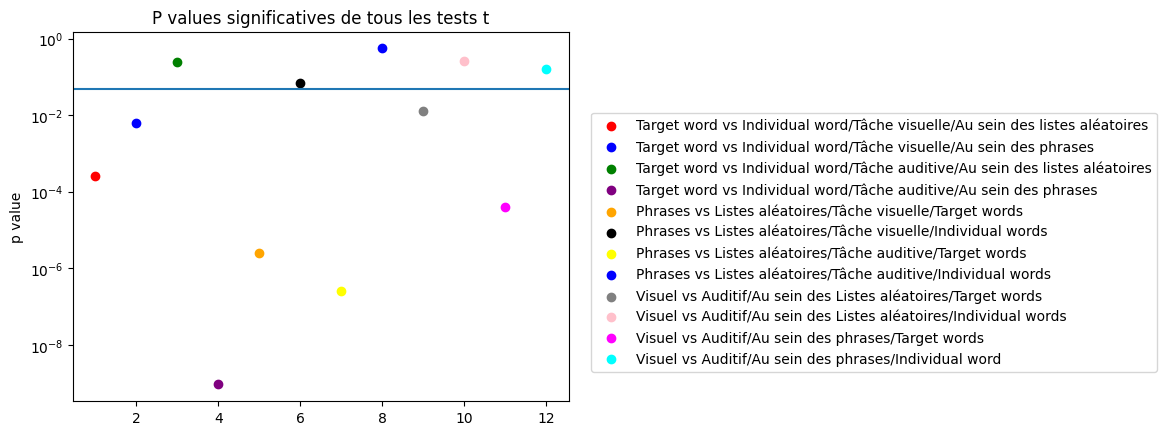
\includegraphics[width=15cm]{p_value_significative.png}
    \caption{Valeurs p significatives des tests t. L'axe des ordonnées est en échelle logarithmique afin de pouvoir distinguer les différentes valeurs}
    \label{fig6.4}
\end{figure}

On peut conclure qu'avec la démarche scientifique que l'on a appliqué et la segmentation temporelle effectuée, le taux d'entropie est majoritairement un bon indicateur pour indexer le complexité linguistique. Toutefois, la dynamique cérébrale ne permet pas de discriminer des conditions expérimentales à chaque fois.
